% Options for packages loaded elsewhere
\PassOptionsToPackage{unicode}{hyperref}
\PassOptionsToPackage{hyphens}{url}
%
\documentclass[
  english,
  man]{apa6}
\usepackage{amsmath,amssymb}
\usepackage{lmodern}
\usepackage{ifxetex,ifluatex}
\ifnum 0\ifxetex 1\fi\ifluatex 1\fi=0 % if pdftex
  \usepackage[T1]{fontenc}
  \usepackage[utf8]{inputenc}
  \usepackage{textcomp} % provide euro and other symbols
\else % if luatex or xetex
  \usepackage{unicode-math}
  \defaultfontfeatures{Scale=MatchLowercase}
  \defaultfontfeatures[\rmfamily]{Ligatures=TeX,Scale=1}
\fi
% Use upquote if available, for straight quotes in verbatim environments
\IfFileExists{upquote.sty}{\usepackage{upquote}}{}
\IfFileExists{microtype.sty}{% use microtype if available
  \usepackage[]{microtype}
  \UseMicrotypeSet[protrusion]{basicmath} % disable protrusion for tt fonts
}{}
\makeatletter
\@ifundefined{KOMAClassName}{% if non-KOMA class
  \IfFileExists{parskip.sty}{%
    \usepackage{parskip}
  }{% else
    \setlength{\parindent}{0pt}
    \setlength{\parskip}{6pt plus 2pt minus 1pt}}
}{% if KOMA class
  \KOMAoptions{parskip=half}}
\makeatother
\usepackage{xcolor}
\IfFileExists{xurl.sty}{\usepackage{xurl}}{} % add URL line breaks if available
\IfFileExists{bookmark.sty}{\usepackage{bookmark}}{\usepackage{hyperref}}
\hypersetup{
  pdftitle={Reproducible analysis of Schroeder \& Epley, 2015: Do you come across as smarter when people read what you say or hear what you say},
  pdfauthor={Celia S. Florea1},
  pdflang={en-EN},
  pdfkeywords={communcation, speech, mental capacity, reproducible analysis},
  hidelinks,
  pdfcreator={LaTeX via pandoc}}
\urlstyle{same} % disable monospaced font for URLs
\usepackage{graphicx}
\makeatletter
\def\maxwidth{\ifdim\Gin@nat@width>\linewidth\linewidth\else\Gin@nat@width\fi}
\def\maxheight{\ifdim\Gin@nat@height>\textheight\textheight\else\Gin@nat@height\fi}
\makeatother
% Scale images if necessary, so that they will not overflow the page
% margins by default, and it is still possible to overwrite the defaults
% using explicit options in \includegraphics[width, height, ...]{}
\setkeys{Gin}{width=\maxwidth,height=\maxheight,keepaspectratio}
% Set default figure placement to htbp
\makeatletter
\def\fps@figure{htbp}
\makeatother
\setlength{\emergencystretch}{3em} % prevent overfull lines
\providecommand{\tightlist}{%
  \setlength{\itemsep}{0pt}\setlength{\parskip}{0pt}}
\setcounter{secnumdepth}{-\maxdimen} % remove section numbering
% Make \paragraph and \subparagraph free-standing
\ifx\paragraph\undefined\else
  \let\oldparagraph\paragraph
  \renewcommand{\paragraph}[1]{\oldparagraph{#1}\mbox{}}
\fi
\ifx\subparagraph\undefined\else
  \let\oldsubparagraph\subparagraph
  \renewcommand{\subparagraph}[1]{\oldsubparagraph{#1}\mbox{}}
\fi
% Manuscript styling
\usepackage{upgreek}
\captionsetup{font=singlespacing,justification=justified}

% Table formatting
\usepackage{longtable}
\usepackage{lscape}
% \usepackage[counterclockwise]{rotating}   % Landscape page setup for large tables
\usepackage{multirow}		% Table styling
\usepackage{tabularx}		% Control Column width
\usepackage[flushleft]{threeparttable}	% Allows for three part tables with a specified notes section
\usepackage{threeparttablex}            % Lets threeparttable work with longtable

% Create new environments so endfloat can handle them
% \newenvironment{ltable}
%   {\begin{landscape}\begin{center}\begin{threeparttable}}
%   {\end{threeparttable}\end{center}\end{landscape}}
\newenvironment{lltable}{\begin{landscape}\begin{center}\begin{ThreePartTable}}{\end{ThreePartTable}\end{center}\end{landscape}}

% Enables adjusting longtable caption width to table width
% Solution found at http://golatex.de/longtable-mit-caption-so-breit-wie-die-tabelle-t15767.html
\makeatletter
\newcommand\LastLTentrywidth{1em}
\newlength\longtablewidth
\setlength{\longtablewidth}{1in}
\newcommand{\getlongtablewidth}{\begingroup \ifcsname LT@\roman{LT@tables}\endcsname \global\longtablewidth=0pt \renewcommand{\LT@entry}[2]{\global\advance\longtablewidth by ##2\relax\gdef\LastLTentrywidth{##2}}\@nameuse{LT@\roman{LT@tables}} \fi \endgroup}

% \setlength{\parindent}{0.5in}
% \setlength{\parskip}{0pt plus 0pt minus 0pt}

% \usepackage{etoolbox}
\makeatletter
\patchcmd{\HyOrg@maketitle}
  {\section{\normalfont\normalsize\abstractname}}
  {\section*{\normalfont\normalsize\abstractname}}
  {}{\typeout{Failed to patch abstract.}}
\patchcmd{\HyOrg@maketitle}
  {\section{\protect\normalfont{\@title}}}
  {\section*{\protect\normalfont{\@title}}}
  {}{\typeout{Failed to patch title.}}
\makeatother
\shorttitle{Semester Project}
\keywords{communcation, speech, mental capacity, reproducible analysis\newline\indent Word count: 882}
\DeclareDelayedFloatFlavor{ThreePartTable}{table}
\DeclareDelayedFloatFlavor{lltable}{table}
\DeclareDelayedFloatFlavor*{longtable}{table}
\makeatletter
\renewcommand{\efloat@iwrite}[1]{\immediate\expandafter\protected@write\csname efloat@post#1\endcsname{}}
\makeatother
\usepackage{csquotes}
\ifxetex
  % Load polyglossia as late as possible: uses bidi with RTL langages (e.g. Hebrew, Arabic)
  \usepackage{polyglossia}
  \setmainlanguage[]{english}
\else
  \usepackage[main=english]{babel}
% get rid of language-specific shorthands (see #6817):
\let\LanguageShortHands\languageshorthands
\def\languageshorthands#1{}
\fi
\ifluatex
  \usepackage{selnolig}  % disable illegal ligatures
\fi
\newlength{\cslhangindent}
\setlength{\cslhangindent}{1.5em}
\newlength{\csllabelwidth}
\setlength{\csllabelwidth}{3em}
\newenvironment{CSLReferences}[2] % #1 hanging-ident, #2 entry spacing
 {% don't indent paragraphs
  \setlength{\parindent}{0pt}
  % turn on hanging indent if param 1 is 1
  \ifodd #1 \everypar{\setlength{\hangindent}{\cslhangindent}}\ignorespaces\fi
  % set entry spacing
  \ifnum #2 > 0
  \setlength{\parskip}{#2\baselineskip}
  \fi
 }%
 {}
\usepackage{calc}
\newcommand{\CSLBlock}[1]{#1\hfill\break}
\newcommand{\CSLLeftMargin}[1]{\parbox[t]{\csllabelwidth}{#1}}
\newcommand{\CSLRightInline}[1]{\parbox[t]{\linewidth - \csllabelwidth}{#1}\break}
\newcommand{\CSLIndent}[1]{\hspace{\cslhangindent}#1}

\title{Reproducible analysis of Schroeder \& Epley, 2015: Do you come across as smarter when people read what you say or hear what you say}
\author{Celia S. Florea\textsuperscript{1}}
\date{}


\authornote{

Celia S. Florea, Department of Psychology, Brooklyn College of the City University of New York.

Correspondence concerning this article should be addressed to Celia S. Florea, 2900 Bedford Avenue, Brooklyn NY. E-mail: \href{mailto:celia.florea99@bcmail.cuny.edu}{\nolinkurl{celia.florea99@bcmail.cuny.edu}}

}

\affiliation{\vspace{0.5cm}\textsuperscript{1} Brooklyn College of the City University of New York}

\abstract{
This is a reproducible report based on a reanalysis of study 4 from Schroeder \& Epley (2015) entitled ``Do you come across as smarter when people read what you say or hear what you say?'' Their analysis and the reproduced analysis here do indeed provide compelling support for their hypothesis speech conveys information about a persons' mental capacity which cannot be capatured in text.
}



\begin{document}
\maketitle

\hypertarget{method}{%
\section{Method}\label{method}}

This report reproduces the analysis from experiment 4 in Schroeder \& Epley (2015). The data were downloaded from the ``open data'' folder for this class, from the file named ``SchroederEpley2015data.csv.'' In experiment 4 Schroeder \& Epley (2015) replicated the results of experiments 1-3 but here enlisted professional recruiters as participants to improve the ecological validity of their experiment.

\hypertarget{participants}{%
\subsection{Participants}\label{participants}}

The participants N=39 (mean age=30.85 years, SD= 6.24, 30 females) in experiment 4 were professional recruiters from fortune 500 companies who had agreed to evaluate potential candidates at the University of Chicago Booth School of Business. The experimenters reached out to 66 recruiters who had attended such a jobs conference at the University of Chicago via email to request their participation in a survey. Of the 66 recruiters contacted, 39 responded and agreed to participate.

\hypertarget{materials}{%
\subsection{Materials}\label{materials}}

The stimuli which were developed for experiment 1, of which a subset were used here in experiment 4, were created from video recordings of MBA students spoken elevator pitches made for potential employers. It was predicted that evaluators would respond more positively to the pitches that they heard rather than those they read, as this would make the candidates appear more thoughtful and intelligent.

The survey then asked participants to rate each potential candidate on 3 dimensions: the candidate's competence (as compared to the average candidate for a similar position), their thoughtfulness, and intelligence. The recruiters were then asked to rate their general impressions of the candidates with questions that probed how much they liked the candidate, how positive and negative their overall impressions were and whether or not they would opt to hire the candidate.

\hypertarget{procedure}{%
\subsection{Procedure}\label{procedure}}

Participants responded to an online survey and were randomly assigned to either listen to recordings of spoken pitches (audio condition) or the same pitch in text (transcript condition) and answered survey questions. The materials were the same as experiment 1 (except that there was no video condition in experiment 4). The survey questions were rated on a likert type scale from 0-10 (e.g.~0 = much less thoughtful, 10 = much more thoughtful).

The recruiters ratings of the job candidates pitches were collapsed into into composite measures of intellect (cronbach's alpha = .92) and general impressions (cronbach's alpha = .93).

\hypertarget{data-analysis}{%
\subsection{Data analysis}\label{data-analysis}}

We used R {[}Version 4.0.2; R Core Team (2020){]} and the R-packages \emph{apaTables} {[}Version 2.0.8; Stanley (2021){]}, \emph{crayon} {[}Version 1.4.0; Csárdi (2017){]}, \emph{csvread} {[}Version 1.2.1; Izrailev (2018){]}, \emph{data.table} {[}Version 1.13.6; Dowle and Srinivasan (2020){]}, \emph{dplyr} {[}Version 1.0.3; Wickham, François, Henry, and Müller (2021){]}, \emph{forcats} {[}Version 0.5.1; Wickham (2021){]}, \emph{ggplot2} {[}Version 3.3.3; Wickham (2016){]}, \emph{ggpmisc} {[}Version 0.3.8.1; Aphalo (2021){]}, \emph{kableExtra} {[}Version 1.3.1; Zhu (2020){]}, \emph{latex2exp} {[}Version 0.5.0; Meschiari (2015){]}, \emph{latexpdf} {[}Version 0.1.6; Bergsma (2018){]}, \emph{pandocfilters} {[}Version 0.1.4; Schwendinger and Hornik (2019){]}, \emph{papaja} {[}Version 0.1.0.9997; Aust and Barth (2020){]}, \emph{purrr} {[}Version 0.3.4; Henry and Wickham (2020){]}, \emph{pwr} {[}Version 1.3.0; Champely (2020){]}, \emph{readr} {[}Version 1.4.0; Wickham, Hester, and Francois (2018){]}, \emph{stringr} {[}Version 1.4.0; Wickham (2019){]}, \emph{tibble} {[}Version 3.0.6; Müller and Wickham (2021){]}, \emph{tidyr} {[}Version 1.1.2; Wickham (2020){]}, \emph{tidyverse} {[}Version 1.3.0; Wickham et al. (2019){]}, and \emph{tinytex} {[}Version 0.31; Xie (2019){]} for all our analyses.

\hypertarget{results}{%
\section{Results}\label{results}}

\begin{verbatim}
##    CONDITION Intellect_Rating
## 1 transcript         3.648148
## 2      audio         5.634921
\end{verbatim}

\begin{verbatim}
##    CONDITION Impression_Rating
## 1 transcript          4.074074
## 2      audio          5.968254
\end{verbatim}

\begin{verbatim}
##    CONDITION Hire_Rating
## 1 transcript    2.888889
## 2      audio    4.714286
\end{verbatim}

\begin{verbatim}
## 
##  Two Sample t-test
## 
## data:  Intellect_Rating by CONDITION
## t = -3.5259, df = 37, p-value = 0.001144
## alternative hypothesis: true difference in means is not equal to 0
## 95 percent confidence interval:
##  -3.1284798 -0.8450652
## sample estimates:
## mean in group transcript      mean in group audio 
##                 3.648148                 5.634921
\end{verbatim}

\begin{verbatim}
## 
##  Two Sample t-test
## 
## data:  Impression_Rating by CONDITION
## t = -2.8508, df = 37, p-value = 0.007091
## alternative hypothesis: true difference in means is not equal to 0
## 95 percent confidence interval:
##  -3.2404752 -0.5478846
## sample estimates:
## mean in group transcript      mean in group audio 
##                 4.074074                 5.968254
\end{verbatim}

\begin{verbatim}
## 
##  Two Sample t-test
## 
## data:  Hire_Rating by CONDITION
## t = -2.6201, df = 37, p-value = 0.01267
## alternative hypothesis: true difference in means is not equal to 0
## 95 percent confidence interval:
##  -3.2370242 -0.4137694
## sample estimates:
## mean in group transcript      mean in group audio 
##                 2.888889                 4.714286
\end{verbatim}

The results of this analysis are consistent with the original authors in that the mean ratings of the professional recruiters were greater in each condition when they heard audio recordings than read the job seekers elevator pitch. As is also the case of studies 1-3, in study 4 the recruiters rated candidates as more intelligent in the audio than transcript condition \(\Delta M = -1.99\), 95\% CI \([-3.13\), \(-0.85]\), \(t(37) = -3.53\), \(p = .001\), likewise their overall impression of the candidates \(\Delta M = -1.89\), 95\% CI \([-3.24\), \(-0.55]\), \(t(37) = -2.85\), \(p = .007\) and the likelihood that they would hire the candidate \(\Delta M = -1.83\), 95\% CI \([-3.24\), \(-0.41]\), \(t(37) = -2.62\), \(p = .013\) was greater in the audio than transcript condition.
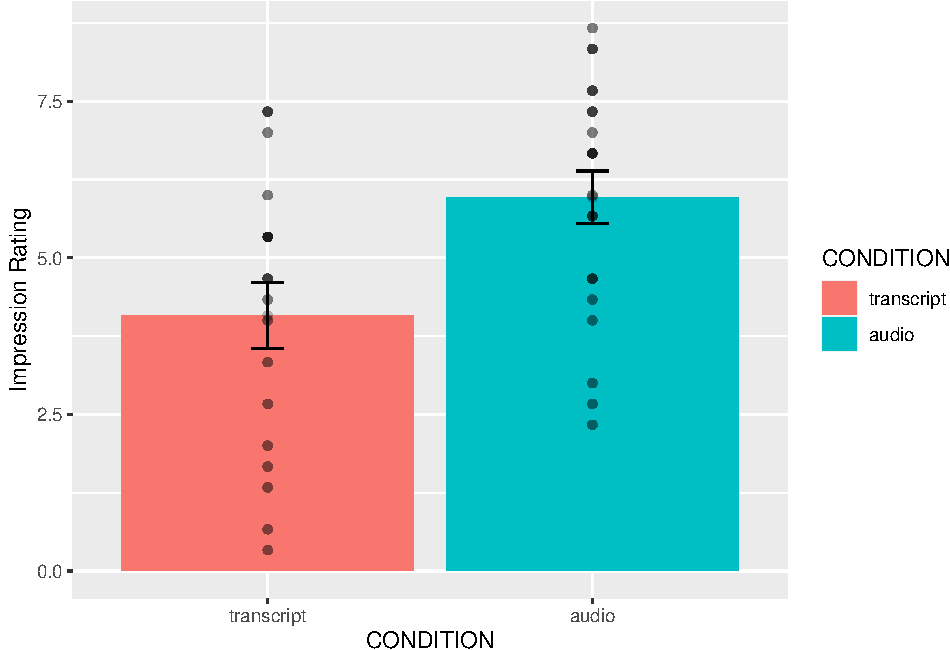
\includegraphics{CSF-semester-project_files/figure-latex/unnamed-chunk-3-1.pdf}
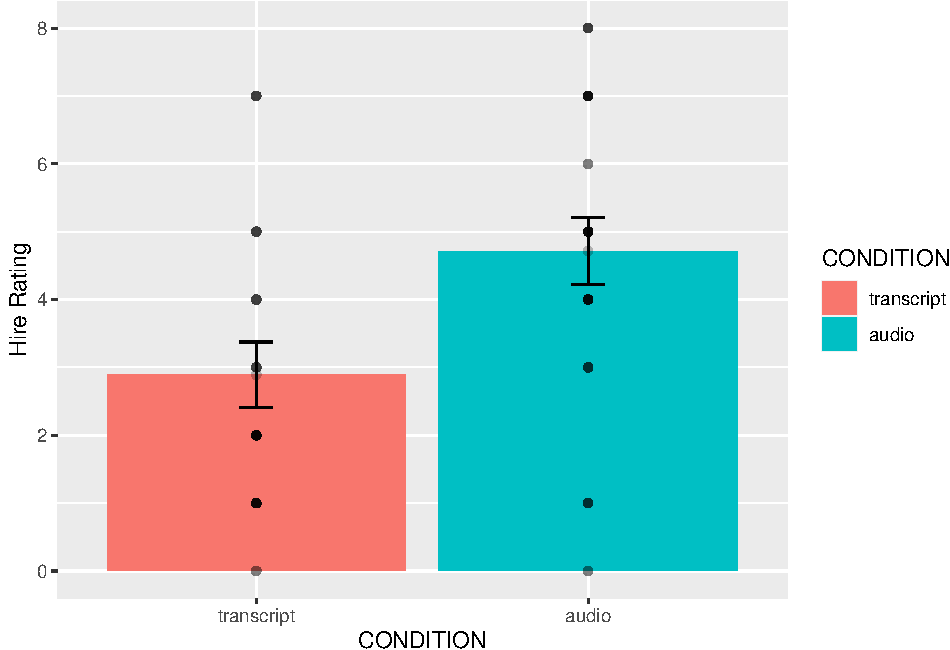
\includegraphics{CSF-semester-project_files/figure-latex/unnamed-chunk-4-1.pdf}
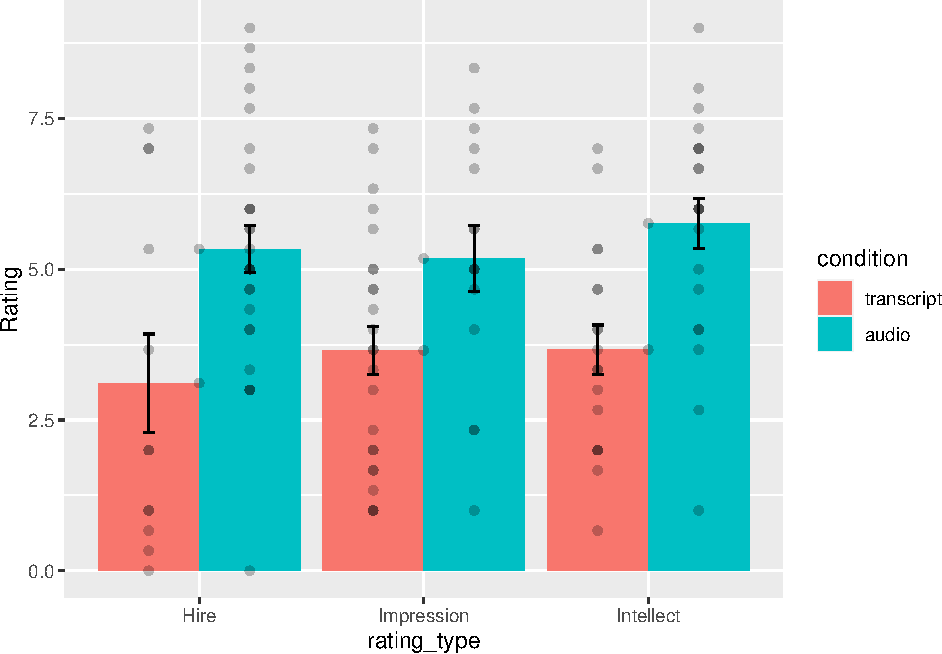
\includegraphics{CSF-semester-project_files/figure-latex/unnamed-chunk-5-1.pdf}

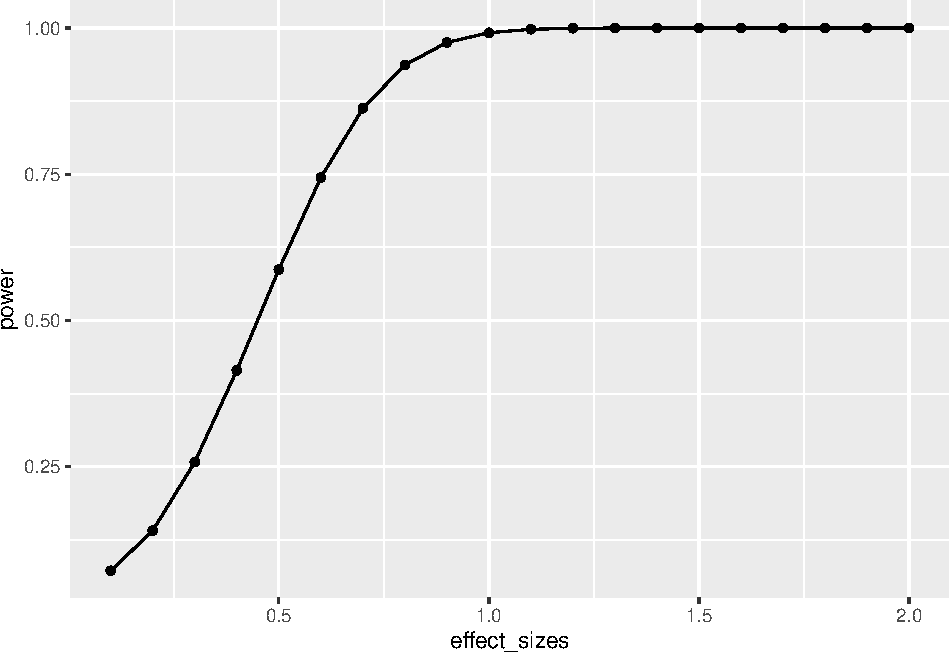
\includegraphics{CSF-semester-project_files/figure-latex/unnamed-chunk-6-1.pdf}

\hypertarget{discussion}{%
\section{Discussion}\label{discussion}}

The results here conform with those found by Schroeder \& Epley (2015) from experiment 4. Recruiters rated candidates more favorably across all dimensions when they heard rather than read candidates' elevator pitches. They argue convincingly that speech allows us to infer information, especially that of another person's mental capacity that cannot be captured in text alone.

\#Powercurve

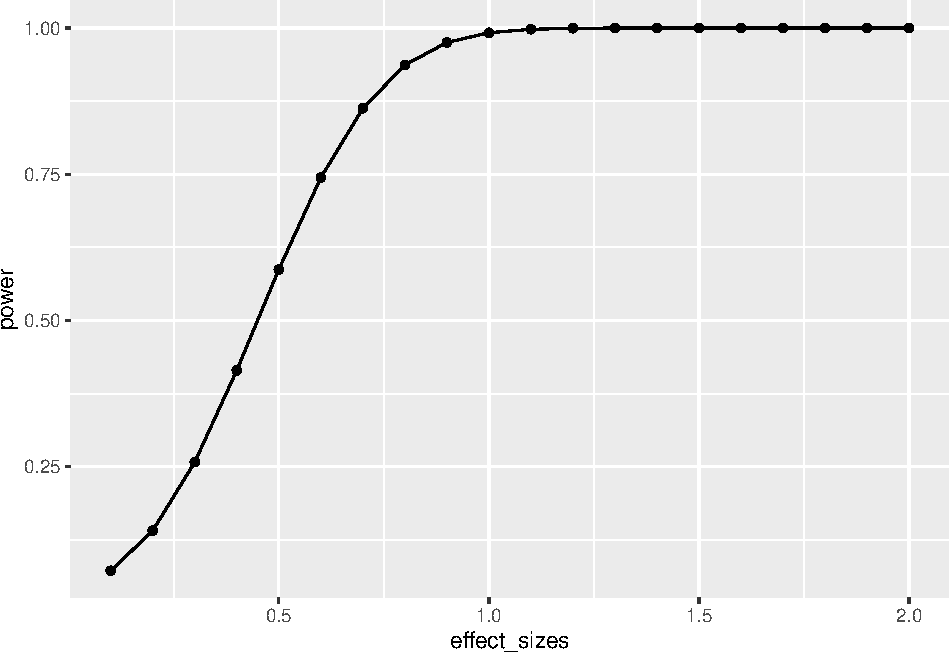
\includegraphics{CSF-semester-project_files/figure-latex/unnamed-chunk-7-1.pdf}

\newpage

\hypertarget{references}{%
\section{References}\label{references}}

Schroeder, J., \& Epley, N. (2015). The Sound of Intellect: Speech Reveals a Thoughtful Mind, Increasing a Job Candidate's Appeal. Psychological Science, 1, 15.

\begingroup
\setlength{\parindent}{-0.5in}
\setlength{\leftskip}{0.5in}

\hypertarget{refs}{}
\begin{CSLReferences}{1}{0}
\leavevmode\hypertarget{ref-R-ggpmisc}{}%
Aphalo, P. J. (2021). \emph{Ggpmisc: Miscellaneous extensions to 'ggplot2'}. Retrieved from \url{https://CRAN.R-project.org/package=ggpmisc}

\leavevmode\hypertarget{ref-R-papaja}{}%
Aust, F., \& Barth, M. (2020). \emph{{papaja}: {Create} {APA} manuscripts with {R Markdown}}. Retrieved from \url{https://github.com/crsh/papaja}

\leavevmode\hypertarget{ref-R-latexpdf}{}%
Bergsma, T. (2018). \emph{Latexpdf: Convert tables to PDF or PNG}. Retrieved from \url{https://CRAN.R-project.org/package=latexpdf}

\leavevmode\hypertarget{ref-R-pwr}{}%
Champely, S. (2020). \emph{Pwr: Basic functions for power analysis}. Retrieved from \url{https://CRAN.R-project.org/package=pwr}

\leavevmode\hypertarget{ref-R-crayon}{}%
Csárdi, G. (2017). \emph{Crayon: Colored terminal output}. Retrieved from \url{https://CRAN.R-project.org/package=crayon}

\leavevmode\hypertarget{ref-R-data.table}{}%
Dowle, M., \& Srinivasan, A. (2020). \emph{Data.table: Extension of `data.frame`}. Retrieved from \url{https://CRAN.R-project.org/package=data.table}

\leavevmode\hypertarget{ref-R-purrr}{}%
Henry, L., \& Wickham, H. (2020). \emph{Purrr: Functional programming tools}. Retrieved from \url{https://CRAN.R-project.org/package=purrr}

\leavevmode\hypertarget{ref-R-csvread}{}%
Izrailev, S. (2018). \emph{Csvread: Fast specialized CSV file loader}. Retrieved from \url{https://CRAN.R-project.org/package=csvread}

\leavevmode\hypertarget{ref-R-latex2exp}{}%
Meschiari, S. (2015). \emph{latex2exp: Use LaTeX expressions in plots}. Retrieved from \url{https://CRAN.R-project.org/package=latex2exp}

\leavevmode\hypertarget{ref-R-tibble}{}%
Müller, K., \& Wickham, H. (2021). \emph{Tibble: Simple data frames}. Retrieved from \url{https://CRAN.R-project.org/package=tibble}

\leavevmode\hypertarget{ref-R-base}{}%
R Core Team. (2020). \emph{R: A language and environment for statistical computing}. Vienna, Austria: R Foundation for Statistical Computing. Retrieved from \url{https://www.R-project.org/}

\leavevmode\hypertarget{ref-R-pandocfilters}{}%
Schwendinger, F., \& Hornik, K. (2019). \emph{Pandocfilters: Pandoc filters for r}. Retrieved from \url{https://CRAN.R-project.org/package=pandocfilters}

\leavevmode\hypertarget{ref-R-apaTables}{}%
Stanley, D. (2021). \emph{apaTables: Create american psychological association (APA) style tables}. Retrieved from \url{https://CRAN.R-project.org/package=apaTables}

\leavevmode\hypertarget{ref-R-ggplot2}{}%
Wickham, H. (2016). \emph{ggplot2: Elegant graphics for data analysis}. Springer-Verlag New York. Retrieved from \url{https://ggplot2.tidyverse.org}

\leavevmode\hypertarget{ref-R-stringr}{}%
Wickham, H. (2019). \emph{Stringr: Simple, consistent wrappers for common string operations}. Retrieved from \url{https://CRAN.R-project.org/package=stringr}

\leavevmode\hypertarget{ref-R-tidyr}{}%
Wickham, H. (2020). \emph{Tidyr: Tidy messy data}. Retrieved from \url{https://CRAN.R-project.org/package=tidyr}

\leavevmode\hypertarget{ref-R-forcats}{}%
Wickham, H. (2021). \emph{Forcats: Tools for working with categorical variables (factors)}. Retrieved from \url{https://CRAN.R-project.org/package=forcats}

\leavevmode\hypertarget{ref-R-tidyverse}{}%
Wickham, H., Averick, M., Bryan, J., Chang, W., McGowan, L. D., François, R., \ldots{} Yutani, H. (2019). Welcome to the {tidyverse}. \emph{Journal of Open Source Software}, \emph{4}(43), 1686. \url{https://doi.org/10.21105/joss.01686}

\leavevmode\hypertarget{ref-R-dplyr}{}%
Wickham, H., François, R., Henry, L., \& Müller, K. (2021). \emph{Dplyr: A grammar of data manipulation}. Retrieved from \url{https://CRAN.R-project.org/package=dplyr}

\leavevmode\hypertarget{ref-R-readr}{}%
Wickham, H., Hester, J., \& Francois, R. (2018). \emph{Readr: Read rectangular text data}. Retrieved from \url{https://CRAN.R-project.org/package=readr}

\leavevmode\hypertarget{ref-R-tinytex}{}%
Xie, Y. (2019). TinyTeX: A lightweight, cross-platform, and easy-to-maintain LaTeX distribution based on TeX live. \emph{TUGboat}, (1), 30--32. Retrieved from \url{http://tug.org/TUGboat/Contents/contents40-1.html}

\leavevmode\hypertarget{ref-R-kableExtra}{}%
Zhu, H. (2020). \emph{kableExtra: Construct complex table with 'kable' and pipe syntax}. Retrieved from \url{https://CRAN.R-project.org/package=kableExtra}

\end{CSLReferences}

\endgroup


\end{document}
